\documentclass[letterpaper,11pt,leqno]{article}
\usepackage{paper}
\usepackage{tikz}
\usepackage{amsmath}
\usepackage{algorithm}
\usepackage{algpseudocode}
\usepackage{booktabs}
\usepackage{listings}
\usepackage{multicol}
% Style for the CUDA code listings (section on the GPU kernels)
\lstdefinestyle{cuda}{
  language=C++,
  morekeywords={__global__, __device__, __shared__, __constant__, __forceinline__,
                __syncthreads, __shfl_up_sync, __shfl_down_sync, size_t},
  basicstyle=\ttfamily\footnotesize,
  keywordstyle=\bfseries\color{DodgerBlue4},
  commentstyle=\itshape\color{black!60},
  numbers=left, numberstyle=\tiny\color{black!45}, numbersep=6pt,
  frame=lines, framesep=4pt, xleftmargin=1.5em,
  breaklines=true, columns=fullflexible, keepspaces=true,
  showstringspaces=false, tabsize=4, captionpos=t
}
\usetikzlibrary{arrows.meta,positioning}
\bibliographystyle{paper}

% Enter paper title to populate PDF metadata:
\hypersetup{pdftitle={Internship report: Reverse Time Migration on GPU}}

% Enter path to BibTeX file with references:
\newcommand{\bib}{paper.bib}

% Enter path to PDF file with figures:
\newcommand{\pdf}{figures.pdf}

\begin{document}

% Enter title:
\title{Internship report}

% Enter authors:
\author{Under the supervision of Mr Kerdioui Hichem\\[8pt]
Marouane Djabri
%
% Enter affiliations and acknowledgements:
\thanks{Marouane Djabri: \'Ecole nationale Sup\'erieure d'Informatique (ESI). I thank the software engineering, geology and HPC teams for their helpful discussions.}}

% Enter date:
\date{September 2026}

% Enter paper URL (can be commented out):
% \paperurl{...}   (the template's own URL; add yours here if wanted)

\begin{titlepage}
\maketitle

% Enter abstract:
This report concludes my internship at ENAGEO. It presents a study and performance analysis of Reverse Time Migration (RTM) on GPU architectures. The goal of the study was to measure how much seismic processing can be accelerated by parallel hardware, while verifying the correctness of the results. On the Marmousi2 benchmark, our CUDA implementation migrates a shot 440 to 540 times faster than a single-core CPU reference, and produces the same image to within floating-point rounding. Profiling shows that the computation is limited by memory bandwidth, which explains which optimizations pay off, and a comparison with the Devito framework separates the performance of the kernels from that of the data management.
\end{titlepage}
% Enter main text:
\section{Presentation of the company}\label{s:company}

\subsection{ENAGEO}
ENAGEO (Entreprise Nationale de G\'eophysique) is the Algerian national
geophysics company. Established in 1981 and headquartered in Hassi Messaoud, it
provides land seismic acquisition services in Algeria and neighbouring countries,
that is, it records in the field the seismic data from which the subsurface is
later imaged. The quality of its services is recognized for the expertise and
field knowledge of its teams.

\subsection{Activities}
Beyond acquisition, ENAGEO's activities cover the whole geophysical chain:
\begin{itemize}
\item \emph{seismic processing}: turning the raw field recordings into images of
  the subsurface, the step studied in this report;
\item \emph{seismic interpretation}: identifying geological structures and
  potential reservoirs in these images;
\item \emph{reservoir characterization}: estimating the physical properties of the
  rocks inside a reservoir;
\item \emph{surface solution services}: topography, geodesy and mapping of the
  terrain and installations;
\item \emph{applied geophysics}: geophysical surveys for engineering and
  environmental purposes;
\item \emph{hydraulic drilling}.
\end{itemize}

\subsection{Mission and vision}
ENAGEO's vision is to build fundamental and interdependent platforms, combining
strategies, workflows and technologies, able to respond to a large variety of
geoscience challenges. Its mission is to be a leading company in the oil and gas
industry, offering a wide range of smart solutions together with its partners.

\subsection{Products and services}

\paragraph{Seismic processing.}
\begin{itemize}
\item Low Velocity Layer (LVL) modelling: characterization of the weathered layer
  near the surface, whose slow and irregular velocities distort the seismic
  signal and must be corrected;
\item 2D/3D Kirchhoff pre-stack time migration (KPSTM) processing;
\item 2D/3D Kirchhoff pre-stack depth migration (KPSDM) processing;
\item velocity model building: estimating the velocity of seismic waves in the
  subsurface, which every migration method, including RTM, requires;
\item seismic data transcription: converting recorded data between storage
  formats and media.
\end{itemize}

\paragraph{Reservoir characterization.}
\begin{multicols}{2}
\begin{itemize}
\item generation of total volumes; % TODO: total volume of what? (e.g. porosity)
\item generation of TOC (Total Organic Carbon) volumes, which indicate the
  organic content, and therefore the hydrocarbon potential, of the source rocks;
\item generation of shale volumes, the proportion of clay-rich rock.
\end{itemize}
\end{multicols}

\paragraph{Surface solution services.}
\begin{multicols}{2}
\begin{itemize}
\item design and creation of geodetic surveys (precise positioning networks);
\item linear and areal topographic surveys;
\item topographic surveys by photogrammetry (measurements from photographs);
\item well and facility positioning;
\item topographic monitoring and control;
\item 3D ``as built'' surveys of facilities, recording their actual geometry after
  construction;
\item subsurface utility detection (buried pipes and cables);
\item geographic database design;
\item map production.
\end{itemize}
\end{multicols}

\paragraph{Geotechnical services.} % TODO: confirm the heading of these two items
In-situ tests (measurements performed directly in the ground) and laboratory tests.

\subsection{Organization and the host department}
% To be written.


\section{Introduction}\label{s:introduction}

\paragraph{Seismic surveying} Seismic surveying is at the heart of oil and gas exploration. It enables geologists, geophysicists and engineers to highlight, interpret and then map features such as structural or stratigraphic traps, where hydrocarbons have accumulated in producible quantities. The workflow starts with data acquisition in the field, followed by processing and interpretation. When needed, the data are reprocessed and interpreted again.

\begin{center}
\begin{tikzpicture}[
    stage/.style={draw, rounded corners=2pt, align=center,
        text width=3cm, minimum height=0.9cm, font=\small},
    flow/.style={-{Stealth}, thick},
    node distance=1.2cm
]
\node[stage] (acquisition) {Data acquisition\\in the field};
\node[stage, right=of acquisition] (processing) {Data processing};
\node[stage, right=of processing] (interpretation) {Interpretation};
\node[stage, below=0.8cm of processing] (reprocessing) {Reprocessing};
\draw[flow] (acquisition) -- (processing);
\draw[flow] (processing) -- (interpretation);
\draw[flow] (interpretation.south) |- node[pos=0.25, right, font=\small] {If needed} (reprocessing.east);
\draw[flow] (reprocessing.north) -- (processing.south);
\end{tikzpicture}
\end{center}

\paragraph{Seismic imaging} Seismic imaging is part of the processing step. It constructs images of the Earth's subsurface from recorded seismic waves, revealing the geometry of geological layers, faults and other structures. It is computationally intensive: it requires processing large amounts of data and performing complex numerical calculations. This report studies how much one of its most demanding methods, Reverse Time Migration (RTM), can be accelerated on GPUs, while verifying that the results stay correct.

\section{Brief description of the seismic imaging process}\label{s:seismic imaging}

\paragraph{Principle.} Seismic imaging relies on the propagation of elastic waves~\citep{Robein2003}. A seismic source (vibrator truck, air gun, dynamite) displaces the particles of the medium, which push on their neighbours, and the disturbance propagates through the subsurface. Where the rock properties change, part of the wave is reflected back to the surface and recorded by receivers. Imaging consists in placing these recorded reflections back at the positions in the subsurface where they occurred.

\paragraph{Migration algorithms.} This placement is done by migration algorithms, which differ in how they describe wave propagation and in the resources they require. \emph{Kirchhoff migration} sums the data along computed travel-time curves; it is efficient, but its accuracy is limited where waves follow complex paths. \emph{One-way wave-equation migration} models propagation mainly in one depth direction, which limits its ability to image turning waves and steep structures. \emph{Reverse Time Migration}, the focus of this report, uses the full two-way wave equation: it propagates the source wavefield forward in time and the recorded data backward in time, then combines the two wavefields to form the image. It handles complex propagation paths and steeply dipping structures, at the price of large computing and memory requirements.

\section{The computational bottleneck of RTM}\label{s:computation bottleneck}

To find where the waves were reflected, RTM simulates the propagation of the source wave \emph{forward} in time, propagates the recorded data \emph{backward} in time from the receivers, and looks for the places where the two wavefields meet at the same instant. The imaging step needs the source wavefield at time $t$, but the receiver wavefield is computed from the last time step down to the first. The two are only available together if the history of the source wavefield is kept, which turns a computation problem into a \emph{memory} problem: gigabytes of snapshots per shot.

\subsection{The RTM algorithm}

Let $P$ be the pressure wavefield on a grid of $N = n_x \times n_z$ points (including the absorbing boundary), $v$ the velocity model, $\Delta t$ the time step, $n_t$ the number of time steps, $w(t)$ the source wavelet, $d_s$ the data recorded for shot $s$, and $k$ the snapshot interval. The Laplacian $\nabla_h^2$ is a centered finite-difference stencil of order 8, and $\omega$ is the absorbing (sponge) taper applied near the edges of the grid.

\begin{algorithm}[!htb]
\caption{Shot-profile Reverse Time Migration with a zero-lag cross-correlation
imaging condition}
\label{alg:rtm}
\begin{algorithmic}[1]
\Require velocity model $v$, shots $s = 1,\dots,n_s$ with recorded data $d_s$
\Ensure migrated image $I$
\State $I \gets 0$
\For{each shot $s = 1,\dots,n_s$}
    \For{$t = 0,\dots,n_t-1$} \Comment{forward propagation of the source}
        \State $P^{\mathrm{next}} \gets \omega\,\bigl(2P - P^{\mathrm{prev}}
               + (v\,\Delta t)^2\,\nabla_h^2 P\bigr)$, add $(v\,\Delta t)^2\,w(t)$ at the source
               \label{alg:forward-update}
        \State \textbf{if} $t \bmod k = 0$ \textbf{then} $S_{t} \gets P$ \Comment{snapshot: the memory cost}
    \EndFor
    \For{$t = n_t-1,\dots,0$} \Comment{backward propagation of the data}
        \State $R^{\mathrm{next}} \gets \omega\,\bigl(2R - R^{\mathrm{prev}}
               + (v\,\Delta t)^2\,\nabla_h^2 R\bigr)$, add $(v\,\Delta t)^2\,d_s(t)$ at the receivers
               \label{alg:backward-update}
        \State \textbf{if} $t \bmod k = 0$ \textbf{then} $I \gets I + S_{t} \cdot R$ \Comment{imaging condition}
    \EndFor
\EndFor
\State \Return $I$
\end{algorithmic}
\end{algorithm}

The cost is concentrated in the two update lines (lines~\ref{alg:forward-update} and~\ref{alg:backward-update}): each is executed $n_t$ times per shot and touches all $N$ grid points.

\subsection{Computational intensity}

One shot performs two full propagations, $W_{\text{shot}} = 2\,N\,n_t$ grid-point updates of about 29 floating-point operations each (order 8). Halving the grid spacing multiplies the number of points by 4 and, through the stability condition, the number of time steps by 2: the work grows as $1/\Delta x^{3}$. Storing one snapshot every $k$ steps requires $M_{\text{snap}} = (n_t/k)\, n_x\, n_z \times 4$ bytes, which grows in the same way. On the Marmousi model with a snapshot every 10 steps, one shot at $\Delta x = 12.5$~m ($0.56$ million points with the boundary, 2\,800 steps) performs $9.0\times10^{10}$ operations, moves 75~GB through memory and stores 0.43~GB of snapshots; at 2.5~m ($10.4$ million points, 14\,000 steps) these become $8.4\times10^{12}$ operations, 7.0~TB and 53~GB.

\paragraph{Arithmetic intensity.} Each update reads the current and previous wavefields and the velocity model and writes the new wavefield: 16 to 24 bytes for about 29 operations, i.e.\ $AI \approx 1.2$ to $1.8$ FLOP/byte. An NVIDIA A40 executes about 37~TFLOP/s but delivers only about 0.7~TB/s from its memory: it needs about 54 operations per byte to keep its arithmetic units busy, 30 to 45 times more than RTM provides. RTM is therefore \emph{memory-bound}: its speed is set by memory bandwidth, not by arithmetic capability. This is why GPUs, whose memory bandwidth is several times that of a CPU (578 against 80~GB/s measured on our platform), are the natural target, and why the optimizations studied here aim at moving fewer bytes rather than computing faster.

\section{Optimization opportunity}

The three nested loops of Algorithm~\ref{alg:rtm} offer parallelism at two levels. \emph{Shots are independent}: each uses its own source and data and only adds its contribution to the image, so shots can run simultaneously on different processors. \emph{Grid points are independent within a time step}: the update of a point at step $t+1$ reads only values of steps $t$ and $t-1$, so all $N$ updates of a step, and all $N$ imaging products, can be computed at the same time. \emph{Only time is sequential}. At 12.5~m, each step offers $5.6 \times 10^{5}$ independent updates: a structure that matches a GPU with thousands of cores.

\section{Methodology and implementation}\label{s:methodology}

\subsection{Experimental setup}

\paragraph{Platform and tools.} The experiments ran on a cloud instance (RunPod) with an NVIDIA A40 GPU (Ampere, 84~SMs, 48~GB, 696~GB/s nominal and 578~GB/s measured bandwidth), 8 cores of an Intel Xeon Gold 6342 and 50~GB of host memory. The engines are written in C++17 with OpenMP and CUDA~12.8; the GPU versions were profiled with NVIDIA Nsight Systems. Nsight Compute could not be used, because the cloud provider blocks access to the GPU performance counters (\texttt{ERR\_NVGPUCTRPERM}): the kernel analysis relies on timelines, measured timings and a model of the memory traffic.

\paragraph{Devito.} Devito~\citep{Louboutin2019Devito, Luporini2020Devito} is an open-source finite-difference framework used in research and industry for seismic imaging. The equations are written symbolically in Python, and Devito generates and compiles optimized code for the target machine (OpenACC on GPUs). We implemented the same RTM with Devito and ran it on exactly the same data and parameters. It serves as an independent check of our images and as a state-of-the-art performance reference.

\paragraph{Dataset.} The velocity model is Marmousi2~\citep{Martin2006Marmousi2}, a benchmark built on a realistic geological section with layered sediments, faults and a salt-like structure. The shot records are synthetic, computed with our reference engine, so that any difference between an engine's image and the reference comes from the engine. Table~\ref{tab:dataset} gives the parameters.

\begin{table}[!htb]
\centering
\caption{Parameters of the Marmousi2 dataset used for the benchmarks.}
\label{tab:dataset}
\begin{tabular}{ll}
\toprule
Parameter              & Value \\
\midrule
Model size             & $17 \times 3.5$~km, $1361 \times 281$ points, $\Delta x = \Delta z = 12.5$~m \\
Shots and receivers    & 12 shots, 341 receivers every 50~m, all at 25~m depth \\
Recording              & $n_t = 2800$ steps of $\Delta t = 1$~ms (2.8~s), Ricker source, $f_0 = 10$~Hz \\
Numerical scheme       & order 8 in space, 2 in time; Cerjan sponge~\citep{Cerjan1985}, 50 cells \\
Snapshots              & one every 10 time steps \\
\bottomrule
\end{tabular}
\end{table}

\paragraph{Correctness criterion.} Every image is compared with the image of the CPU reference. An engine is accepted when the relative $L_2$ difference is below $10^{-5}$ and the correlation above $0.9999$, which corresponds to floating-point rounding.

\subsection{Implementation}

All engines live in one C++ code base, share the same inputs and outputs, and are selected by name at run time. Every run's image is compared automatically with the reference: no engine is timed without being checked.

\begin{itemize}
\item \emph{CPU reference}: a direct, single-threaded translation of Algorithm~\ref{alg:rtm}. It defines the expected image and is reproducible bit for bit (verified on AMD and Intel processors).
\item \emph{Optimized CPU engine}: multi-threaded with OpenMP, vectorized, with the absorbing boundary merged into the stencil loop. It produces the same image bit for bit and is the fair CPU baseline.
\item \emph{GPU versions v0 to v4}: each version changes one aspect of the previous one, so that the effect of every optimization is measured on its own (Section~\ref{s:kernels}).
\end{itemize}

\subsection{The GPU kernels, version by version}\label{s:kernels}

\paragraph{Common structure.} The wavefields are stored with depth as the fastest index. Each GPU thread updates one grid point, in blocks of $32 \times 8$ threads: the 32 threads along $z$ form one warp and read 32 consecutive floats in a single \emph{coalesced} memory transaction. The stencil coefficients live in constant memory. The time loop runs on the CPU, which launches the kernels of each step; the three wavefields stay in GPU memory and are exchanged by swapping pointers, and only the final image is copied back to the host.

\paragraph{Version 0: the baseline.} Version~0 translates the reference directly, with one kernel per operation: the stencil kernel computes the Laplacian from the 8 neighbours in each direction and the new wavefield, a second kernel applies the absorbing boundary to the whole grid, and on imaging steps a third kernel accumulates the image. Since neighbouring values are mostly served by the GPU caches, the stencil moves about 16~bytes per point (read $P$, $P^{\mathrm{prev}}$, $(v\Delta t)^2$, write $P^{\mathrm{next}}$), and the boundary kernel 20~bytes more: 36~bytes per point and per step.

\paragraph{Version 1: absorbing boundary merged into the stencil.} The thread that computes $P^{\mathrm{next}}$ already holds it and $P$ in registers; version~1 applies the damping there, before writing (\texttt{p\_cur[i] = pc\_i * w; p\_next[i] = pn\_i * w;}). The separate kernel disappears, the traffic falls from 36 to 24~bytes per point, and the image is unchanged, since the damping coefficient is exactly~1 where sources and receivers are injected.

\paragraph{Version 2: imaging merged into the backward stencil.} On imaging steps, the backward stencil kernel accumulates $I \gets I + S_t \cdot R$ with the value it has just computed, instead of a separate kernel reading $R$ again (receiver positions are finished after the data injection). The gain is small: imaging happens once every 10 steps.

\paragraph{Version 3: shared memory.} Each block copies its $32 \times 8$ points of $P$, plus a halo of 4 points on each side, into fast on-chip \emph{shared memory}, from which every neighbour is then read.

\paragraph{Version 4: warp shuffles.} The vertical neighbours of a point are held by other threads of the same warp; version~4 reads them from their registers with \emph{shuffle} instructions and keeps the tile only for the horizontal neighbours.

\begin{table}[H]
\centering
\caption{The five GPU versions: kernels launched per time step, estimated memory traffic, and measured GPU time per step (Nsight Systems, NVIDIA A40, 67\,200 time steps).}
\label{tab:kernels-summary}
\begin{tabular}{llccc}
\toprule
Version & Change & Kernels/step & Bytes/point & Time/step \\
\midrule
v0 & one thread per point, one kernel per operation & 3.05 & 36 & 33.3~\textmu s \\
v1 & absorbing boundary merged into the stencil    & 2.05 & 24 & 27.2~\textmu s \\
v2 & imaging merged into the backward stencil      & 2.05 & 24 & 27.3~\textmu s \\
v3 & neighbours read from shared memory            & 2.05 & 24 & 28.4~\textmu s \\
v4 & vertical neighbours via warp shuffles         & 2.05 & 24 & 28.8~\textmu s \\
\bottomrule
\end{tabular}
\end{table}

\section{Results and performance analysis}\label{s:results}

All measurements come from the A40 platform and the dataset of Table~\ref{tab:dataset} unless stated otherwise.
\subsection{The migrated images and their correctness}

\paragraph{The image.} Figure~\ref{fig:image} shows the migrated Marmousi2 section after illumination compensation and Laplacian filtering, which remove the low-frequency artefacts of the cross-correlation imaging condition. The structures of the model are visible: layered sediments on the left, faulted blocks dipping through the center between 8 and 11~km, a strong reflector at about 2.3~km depth. The twelve arcs along the top are the acquisition footprint of the twelve shots.

\begin{figure}[H]
\centering
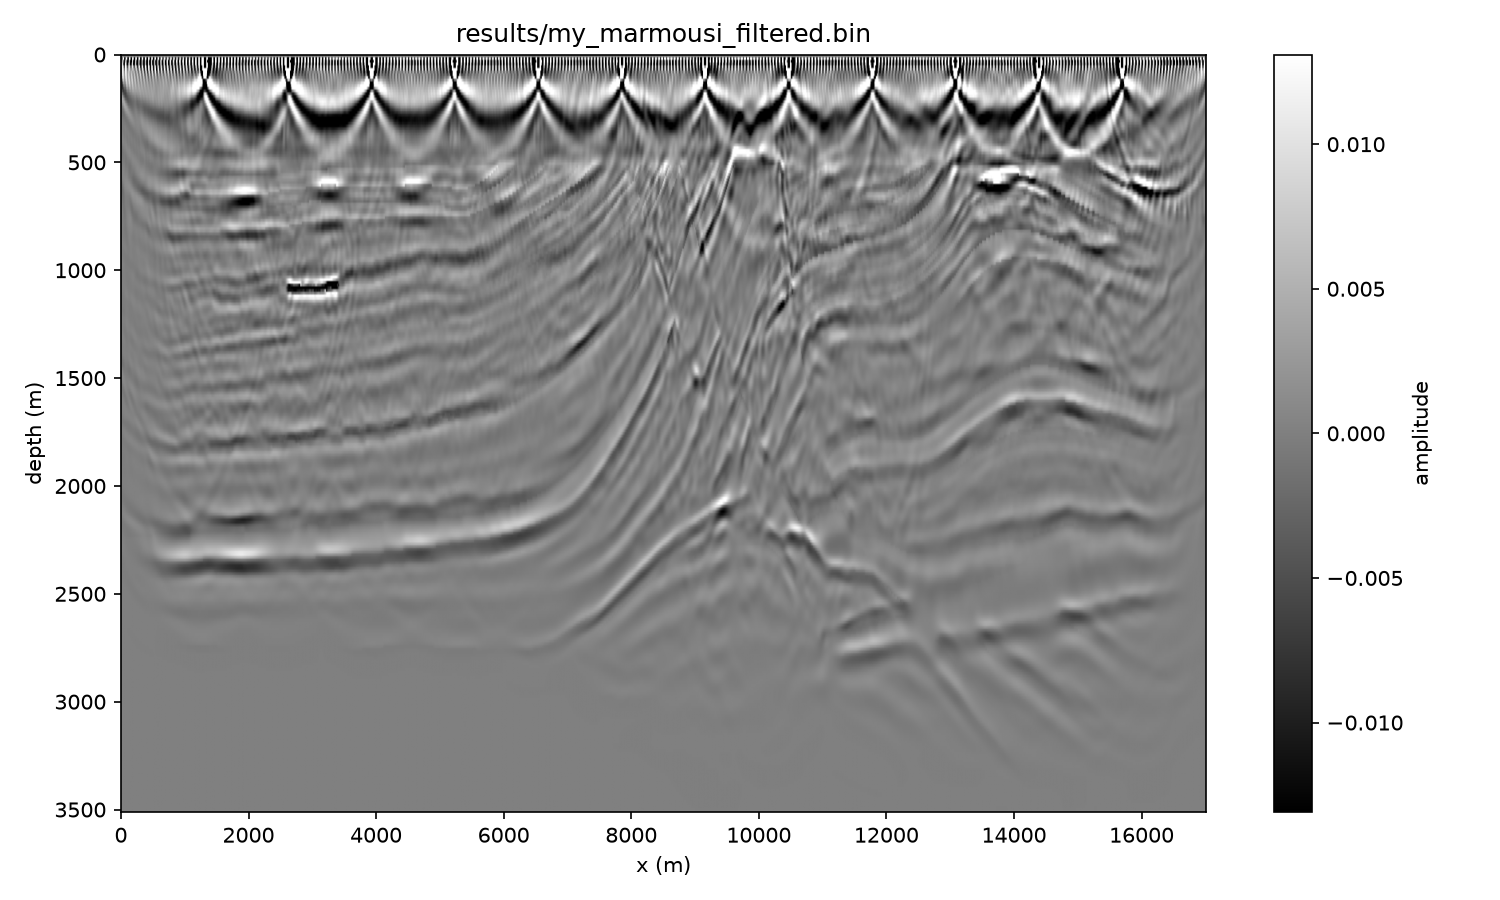
\includegraphics[width=0.72\linewidth]{figures/image_final.png}
\caption{Migrated Marmousi2 section (12 shots, $\Delta x = 12.5$~m), after
illumination compensation and Laplacian filtering.}
\label{fig:image}
\end{figure}

\paragraph{Every version produces the same image.} Table~\ref{tab:correctness} compares each engine's image with the reference on two GPUs of different generations. The optimized CPU engine is bit-identical. The GPU images differ by a relative $L_2$ norm of about $10^{-5}$, with a correlation of exactly 1: the signature of floating-point rounding, since the GPU compiler contracts a multiplication and an addition into one fused multiply-add, and small differences accumulate over the 67\,200 time steps. A programming error produces differences of $10^{-3}$ or more. On the Blackwell GPU, v3 and v4 land just above the $10^{-5}$ threshold; the largest local difference is $0.53\times10^{-5}$ of the image's peak, near the shallow sources, with no structure resembling a reflector.

\begin{table}[!htb]
\centering
\caption{Difference between each engine's image and the CPU reference image.}
\label{tab:correctness}
\begin{tabular}{lccc}
\toprule
       & \multicolumn{2}{c}{Relative $L_2$ difference} & \\
\cmidrule(lr){2-3}
Engine & A40 (Ampere) & RTX PRO 6000 (Blackwell) & Correlation \\
\midrule
Optimized CPU & 0 (bit-identical) & ---                  & 1 \\
v0            & $4.3\times10^{-6}$ & $4.3\times10^{-6}$  & 1.0000000 \\
v1            & $4.2\times10^{-6}$ & $7.3\times10^{-6}$  & 1.0000000 \\
v2            & $4.6\times10^{-6}$ & $7.5\times10^{-6}$  & 1.0000000 \\
v3            & $8.5\times10^{-6}$ & $1.45\times10^{-5}$ & 1.0000000 \\
v4            & $6.7\times10^{-6}$ & $1.06\times10^{-5}$ & 1.0000000 \\
\bottomrule
\end{tabular}
\end{table}

\paragraph{Comparison with Devito.} Devito's image of the same data shows the same reflectors at the same positions: correlation $0.95$ after the display filter, $0.69$ on the raw images, where the two codes' different amplitude scaling weighs most. The remaining differences come from independent choices (absorbing boundary, source interpolation); the agreement confirms that our reference solves the intended problem.

\subsection{Speed-up over the CPU}

Table~\ref{tab:speedup} gives the time needed to migrate the 12 shots, from the first to the last shot, including all data transfers.

\begin{table}[!htb]
\centering
\caption{Time to migrate the 12-shot Marmousi dataset, throughput, and
speed-up relative to the two CPU engines (Xeon Gold 6342, 8 cores; NVIDIA A40).}
\label{tab:speedup}
\begin{tabular}{lrrrrr}
\toprule
       &           &          & Throughput & \multicolumn{2}{c}{Speed-up vs} \\
\cmidrule(lr){5-6}
Engine & Total (s) & Shot (s) & (Gpts/s)   & CPU ref. & opt.\ CPU \\
\midrule
CPU ref.\ (1 core)       & 1016.5 & 84.7   & 0.037 & 1         & ---  \\
Opt.\ CPU (8 cores)      & 498.9  & 41.6   & 0.075 & 2.0       & 1    \\
Devito (GPU)             & 10.2   & 0.853  & 3.7   & 99        & 49   \\
Ours, v0                 & 2.32   & 0.193  & 16.2  & 439       & 215  \\
Ours, v1                 & 2.13   & 0.178  & 20.0  & 476       & 234  \\
Ours, v2                 & 1.88   & 0.156  & 20.0  & 542       & 266  \\
Ours, v3                 & 1.95   & 0.162  & 19.3  & 523       & 256  \\
Ours, v4                 & 1.97   & 0.164  & 19.0  & 516       & 253  \\
\bottomrule
\end{tabular}
\end{table}

A shot that takes 84.7~s on one CPU core, and 41.6~s on 8 cores, takes 0.16 to 0.19~s with our GPU versions: a speed-up of \textbf{440 to 540} over the reference and \textbf{215 to 266} over the optimized CPU engine. Devito, on the same GPU, is 99 and 49 times faster. The CPU baseline is an 8-core cloud instance, so these speed-ups compare one A40 with this instance. v2 appears faster than v1 only in the total: their propagation times are equal (1.87~s), and v1 spends extra time once before the first shot.

\subsection{Where the GPU time goes}\label{s:profile}

Dividing the total time of each kernel recorded by Nsight Systems by the 67\,200 time steps gives the cost of one time step (Figure~\ref{fig:step-breakdown}).

\begin{figure}[!htb]
\centering
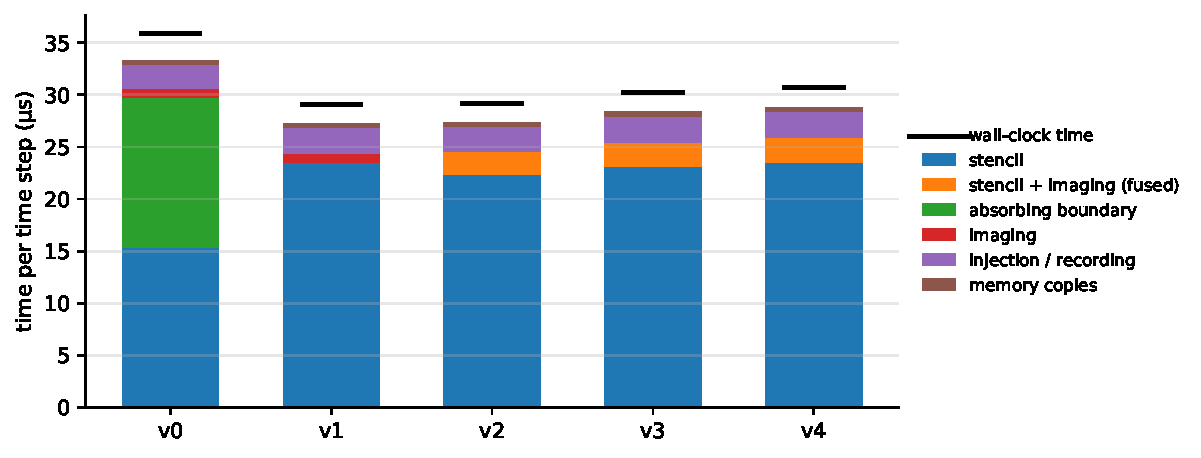
\includegraphics[width=0.55\linewidth]{figures/step_breakdown.pdf}
\caption{GPU time of one time step for each version, broken down by kernel
(Nsight Systems, NVIDIA A40). The black marks give the wall-clock time per step.}
\label{fig:step-breakdown}
\end{figure}

\paragraph{Merging kernels is the decisive optimization.} In v0, the separate absorbing-boundary kernel costs 14.4~\textmu s per step, almost as much as the stencil (15.4~\textmu s), although it performs one multiplication per point: both kernels are limited by memory traffic. Merging them (v1) removes one full pass over the grid: 23.5~\textmu s instead of 29.8, and the time per step drops from 33.3 to 27.2~\textmu s ($-18\,\%$).

\paragraph{Shared memory and shuffles bring nothing.} At 20~billion updates per second and 24~bytes per update, v1 already moves about 83\,\% of the measured bandwidth. v3 and v4 reduce repeated reads of neighbouring values, but these reads were served by the caches: they add instructions and synchronization without reducing the traffic that limits the kernel, and are slightly slower (28.4 and 28.8~\textmu s).

\paragraph{The CPU barely keeps up.} Launching the kernels of a step costs the CPU about 22~\textmu s, against 27~\textmu s of GPU work; the GPU is busy 93 to 94\,\% of the time.

\section{Scaling the workload}\label{s:scaling-section}

The Marmousi dataset is small by industrial standards (0.56 million points, 0.16~s per shot on the GPU). To study realistic sizes, the same model was resampled from 12.5~m down to 1.25~m, the way the workload grows in production. The source frequency is raised in proportion ($f_0 = 10~\text{Hz} \times 12.5/\Delta x$) so that every grid resolves the wave with the same accuracy, the time step is reduced for stability, and every dataset records 2.8~s. Each halving of $\Delta x$ multiplies the work per shot by 8: the finest grid represents about 700 times the work of the original (Table~\ref{tab:scaling}). The snapshot interval is kept at 10 \emph{time steps}: a first campaign with a fixed 10~ms interval aliased the images at fine grids (correlation $0.36$ between the 5~ms and 10~ms images at 2.5~m) and was corrected.

\subsection{Throughput as the grid grows}\label{s:scaling}

\begin{table}[!htb]
\centering
\caption{The scaled datasets and the time per shot and throughput of the two codes (NVIDIA A40). Memory: snapshots, one every 10 time steps. OOM: the run exceeded the available memory.}
\label{tab:scaling}
\begin{tabular}{rrrrrrrr}
\toprule
 & & & & \multicolumn{2}{c}{Ours, v1} & \multicolumn{2}{c}{Devito (GPU)} \\
\cmidrule(lr){5-6}\cmidrule(lr){7-8}
$\Delta x$ (m) & $n_t$ & Points & Memory & s/shot & Gpts/s & s/shot & Gpts/s \\
\midrule
12.5 & 2\,800  & 0.38 M & 0.4 GiB  & 0.156 & 20.1 & 0.853 & 3.7 \\
6.25 & 5\,600  & 1.5 M  & 3.2 GiB  & 0.994 & 21.1 & 3.59  & 5.8 \\
5    & 7\,000  & 2.4 M  & 6.2 GiB  & 1.83  & 21.6 & 6.61  & 5.9 \\
3.75 & 9\,334  & 4.2 M  & 14.7 GiB & 4.08  & 22.1 & 12.7  & 7.0 \\
2.5  & 14\,000 & 9.5 M  & 49.7 GiB & 13.0  & 22.4 & OOM   & --- \\
1.25 & 28\,000 & 38 M   & 397 GiB  & 97.9  & 22.8 & OOM   & --- \\
\bottomrule
\end{tabular}
\end{table}

\begin{figure}[!htb]
\centering
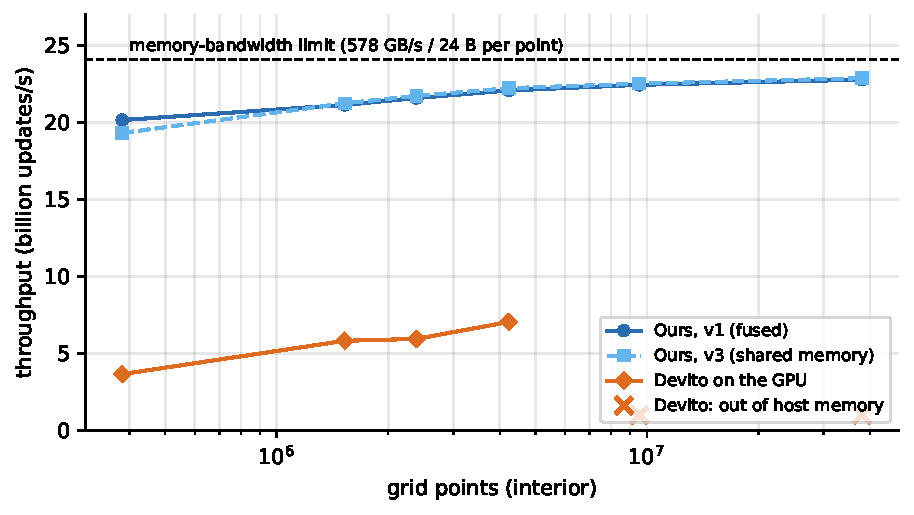
\includegraphics[width=0.55\linewidth]{figures/throughput_vs_size.pdf}
\caption{Throughput as a function of the number of grid points (NVIDIA A40).
The dashed line is the limit set by the measured memory bandwidth.}
\label{fig:throughput-size}
\end{figure}

\paragraph{Our engine reaches the bandwidth limit.} As the work grows by a factor of 700, the time per shot grows by only 630: the throughput \emph{increases} from 20.1 to 22.8~billion updates per second, because the fixed cost of launching kernels becomes negligible. At 24~bytes per update, the kernel then moves about 550~GB/s, $95\,\%$ of the measured bandwidth (Figure~\ref{fig:throughput-size}). v3 runs at the same speed as v1 on every grid, even at 38~million points, far beyond the 6~MB cache.

\paragraph{The stencil order costs nothing.} At 2.5~m, raising the order from 4 to 12 leaves our throughput unchanged (22.4, 22.4 and 22.6~Gpts/s), although it triples the arithmetic: the most direct signature of a memory-bound kernel. Devito slows down at high orders (16.0 to 12.0~Gpts/s from order 4 to 16).

\subsection{The memory limit}

\begin{figure}[!htb]
\centering
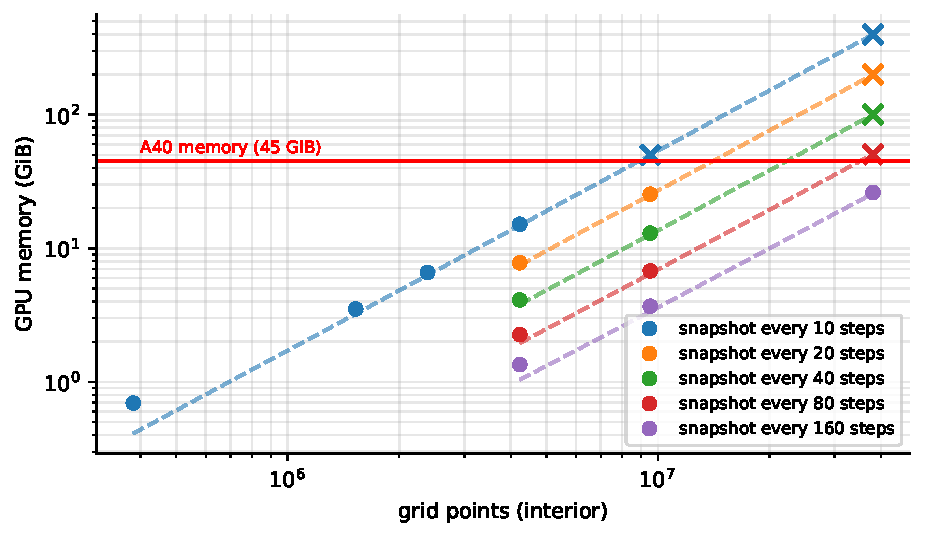
\includegraphics[width=0.52\linewidth]{figures/capacity.pdf}
\caption{GPU memory needed as a function of the grid size, for several snapshot
intervals. Dots: measured. Dashed lines: model. Crosses: runs that exceeded the
memory of the A40 (red line).}
\label{fig:capacity}
\end{figure}

The measured memory follows the model (Figure~\ref{fig:capacity}): with a snapshot every 10 steps it grows as $1/\Delta x^{3}$, from 0.7~GiB at 12.5~m to 15.2~GiB at 3.75~m. At 2.5~m it would need about 50~GiB, more than the 45~GiB available: this is the limit of one A40. Saving fewer snapshots moves the limit, at a price. At 3.75~m, one snapshot every 20 steps leaves the image unchanged (correlation $0.9999986$) for half the memory; every 40 steps the correlation falls to $0.86$, and beyond, the image is destroyed ($0.47$ and $0.43$), because the snapshots no longer sample the highest frequencies (aliasing). At 1.25~m, only one snapshot every 160 steps fits: problems of this size need several GPUs, or techniques such as checkpointing or wavefield compression. Devito keeps its snapshots in host memory instead, so its limit is the 50~GB of RAM of the machine.

\subsection{Impact on a seismic survey}

Projected to 1000 shots at $\Delta x = 2.5$~m (CPU times extrapolated from 12.5~m), a survey would take 2180 hours (91 days) with the CPU reference and 1073 hours (45 days) with the optimized CPU engine, against \textbf{3.7 hours} on one A40 with our engine (5.1 with Devito) and less than an hour on 8 GPUs. For a processing team, this is the difference between weeks and a working day.

\section{Devito versus our engine: faster kernels, slower pipeline}\label{s:devito}

End to end, our engine is three to five times faster than Devito. Nsight Systems separates the time spent computing from the rest, and this separation reverses the conclusion: \emph{Devito's stencil kernel is faster than ours}, by 7\,\% at 12.5~m and by 23 to 29\,\% from 6.25~m onwards (Figure~\ref{fig:devito-kernels}a): at 3.75~m, one time step takes 165.6~\textmu s with Devito against 209.7~\textmu s with our v1 kernel (28.9 against 22.8~Gpts/s).

\paragraph{Devito's kernel moves fewer bytes per point.} Our kernel reproduces the CPU reference exactly, which damps both wavefields at every step: it writes $P$ and $P^{\mathrm{next}}$, 24~bytes per point. Devito damps only the new wavefield and writes only $P^{\mathrm{next}}$: 20~bytes. The ratio $24/20 = 1.2$ is close to the ratio of the kernel times at 3.75~m ($1.27$), and both kernels run at the bandwidth limit ($22.8 \times 24 \approx 550$ and $28.9 \times 20 \approx 580$~GB/s).

\begin{figure}[!htb]
\centering
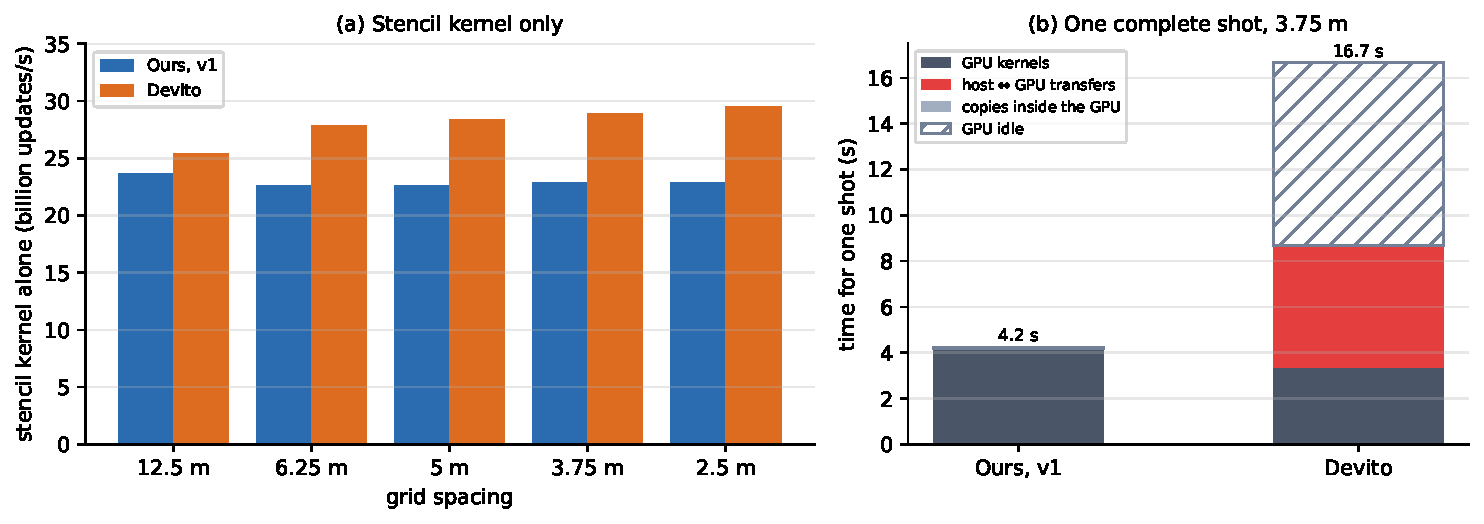
\includegraphics[width=0.75\linewidth]{figures/devito_kernels_vs_end_to_end.pdf}
\caption{(a) Throughput of the stencil kernel alone: Devito is faster on every
grid. (b) One complete shot at 3.75~m, as recorded by Nsight Systems: our GPU
computes almost all the time, while Devito's GPU spends most of the shot
transferring data or idle.}
\label{fig:devito-kernels}
\end{figure}

\paragraph{Devito's pipeline moves the saved wavefield over PCIe.} Of our 4.2~s shot at 3.75~m, 4.1~s are spent in kernels, and almost nothing crosses the host--GPU link. Devito, in its default configuration, keeps the saved wavefield (17.9~GB per shot at 3.75~m) in host memory: Nsight Systems records 55~GB of transfers per shot at 10 to 12~GB/s, about 50 times slower than the GPU memory: 5.3~s per shot, more than Devito's kernels (3.4~s), and the GPU is idle for much of the rest. This is consistent with its lower power draw (115 against 241~W at 3.75~m) and its failure at 2.5~m for lack of host memory.

\paragraph{What this comparison teaches.} Damping only the new wavefield would cut our traffic by 20\,\%; keeping the saved wavefield in GPU memory would remove most of Devito's transfers. The end-to-end ranking reflects data management choices, not the quality of the generated code.

\section{Conclusion}\label{s:conclusion}

\paragraph{Main findings.} \emph{The results are correct}: every GPU version reproduces the reference image to within floating-point rounding (relative difference below $1.5\times10^{-5}$ on two GPU generations), and Devito images the same reflectors. \emph{The GPU changes the scale of the problem}: a shot is migrated 440 to 540 times faster than with the CPU reference and 215 to 266 times faster than with the optimized CPU engine, and a 1000-shot survey at 2.5~m goes from 91 days to 3.7 hours. \emph{RTM is limited by memory bandwidth}: the kernels use up to 95\,\% of the measured bandwidth and less than 2\,\% of the arithmetic capability, so merging kernels is the only clear gain ($-18\,\%$ per step), while shared memory, warp shuffles and higher stencil orders change nothing. \emph{Memory, not speed, limits the problem size}: one A40 reaches its limit between 3.75 and 2.5~m. Finally, Devito's faster kernel but slower pipeline shows that \emph{kernels and data management are separate problems}.

\paragraph{Limitations and future work.} The GPU counters were not accessible, the problem is 2D and acoustic, the data are synthetic, and a single GPU was used. Next steps: 20~bytes per point, CUDA Graphs against the launch overhead, checkpointing or compression and several GPUs against the memory limit, and 3D.

More generally, this work shows that the performance of a seismic imaging code on a GPU depends less on the arithmetic it performs than on the data it moves: the number of bytes per grid point, and where the saved wavefield lives.

\bibliography{\bib}

\end{document}
